\documentclass[output=paper,colorlinks,citecolor=brown]{langscibook} 

\newcommand*{\fullref}[1]{\hyperref[{#1}]{\autoref*{#1}: \nameref*{#1}}} % One single link

%dependencias para desenhar árvores sintáticas
\usepackage{tikz}
\usepackage{tikz-dependency}
%\usepackage{python}
%\usepackage{minted} %\begin{minted}{python}
\usepackage{longtable}

%nome da section no header de cada página
%\usepackage{fancyhdr}
%\pagestyle{fancy}
%\fancyhf{}
%\fancyhead[L]{\rightmark}
%\fancyhead[R]{\thepage}
%\renewcommand{\headrulewidth}{0pt}
\usepackage{dirtytalk}

\bibliography{localbibliography.bib}

\author{Elvis de Souza\affiliation{PUC-Rio, Brasil}\and Tatiana Cavalcanti\and Aline Silveira\and Wograine Evelyn\and Cláudia Freitas}
\title{Documentação UD em português\\
(e para língua portuguesa)}
\abstract{O projeto Universal Dependencies \citep{mcdonald2013universal} apresenta um tagset e uma gramática. Isso significa dizer que, para além de um conjunto de etiquetas que correspondem às classes da Gramática Tradicional (objeto, sujeito etc.), o UD também faz diversas escolhas que diferem da GT. Nesse documento, apresentamos a documentação detalhadas e as escolhas linguísticas relativas ao processo de revisão do material UD em Português. Considerando que UD funciona como uma espécie de segunda língua gramatical, partimos, sempre que possível, das categorias e análises de GT, e não de UD. Os exemplos de frases e as listas foram retirados do corpus \href{https://github.com/UniversalDependencies/UD\_Portuguese-Bosque}{Bosque-UD} (\citet{rademaker2017universal}) versão 2.5.}

% add all extra packages you need to load to this file  
\usepackage{tabularx} 

%%%%%%%%%%%%%%%%%%%%%%%%%%%%%%%%%%%%%%%%%%%%%%%%%%%%
%%%                                              %%%
%%%           Examples                           %%%
%%%                                              %%%
%%%%%%%%%%%%%%%%%%%%%%%%%%%%%%%%%%%%%%%%%%%%%%%%%%%% 
%% to add additional information to the right of examples, uncomment the following line
% \usepackage{jambox}
%% if you want the source line of examples to be in italics, uncomment the following line
% \renewcommand{\exfont}{\itshape}
\usepackage{langsci-optional}
\usepackage{langsci-gb4e}  
\makeatletter
\let\thetitle\@title
\let\theauthor\@author 
\makeatother

\newcommand{\togglepaper}[1][0]{ 
%   \bibliography{../localbibliography}
  \papernote{\scriptsize\normalfont
    \theauthor.
    \thetitle. 
    To appear in: 
    Change Volume Editor \& in localcommands.tex 
    Change volume title in localcommands.tex
    Berlin: Language Science Press. [preliminary page numbering]
  }
  \pagenumbering{roman}
  \setcounter{chapter}{#1}
  \addtocounter{chapter}{-1}
}

\begin{document}

\maketitle

\addtocontents{toc}{\protect\hypertarget{toc}{}}

\tableofcontents

\chapter{Formato UD}\label{sec:formatoud}

\hyperlink{toc}{Ir para tabela de conteúdos\\}

Os treebanks adaptados para a gramática UD são disponibilizados no formato CoNLL-U, em que há um token por linha. Cada anotação de cada token, por sua vez, é disposta em uma coluna, sendo 10 colunas ao todo. Cada token tem a configuração conforme a \fullref{tab:colunasUD}, com uma tabulação (\textit{Tab}) separando as colunas. Colunas sem nenhum valor devem, necessariamente, ser preenchidas com \textit{underline}, conforme diretivas da página do \href{https://universaldependencies.org/format}{formato CoNLL-U} (acesso em 28 de outubro de 2019).

\begin{table}
    \centering
    \begin{tabular}{c c c c c c c c c c}
        id & word & lemma & upos & xpos & feats & dephead & deprel & deps & misc\\
    \end{tabular}
    \caption{Colunas do formato UD 2.0}
    \label{tab:colunasUD}
\end{table}

\section{Princípios}\label{sec:principios}

	De \href{https://universaldependencies.org/introduction.html}{Página do Universal Dependencies} (acesso em 28 de outubro de 2019).
	
	What is needed for UD to be successful?
	The secret to understanding the design and current success of UD is to realize that the design is a very subtle compromise between approximately 6 things:
	
	\begin{enumerate}
		\item UD needs to be satisfactory on linguistic analysis grounds for individual languages.
		\item UD needs to be good for linguistic typology, i.e., providing a suitable basis for bringing out cross-linguistic parallelism across languages and language families.
		\item UD must be suitable for rapid, consistent annotation by a human annotator.
		\item UD must be suitable for computer parsing with high accuracy.
		\item UD must be easily comprehended and used by a non-linguist, whether a language learner or an engineer with prosaic needs for language processing. We refer to this as seeking a habitable design, and it leads us to favor traditional grammar notions and terminology.
		\item UD must support well downstream language understanding tasks (relation extraction, reading comprehension, machine translation, …).
	\end{enumerate}

\section{Colunas/anotações}\label{sec:colunas}



\begin{enumerate}
    \item “id” corresponde ao número do token, em ordem crescente;
    \item “word”, à palavra tal como aparece na frase (exceto no caso de contração, como “da”, em que a palavra será desmembrada nos tokens “de” e “a”);
    \item “lemma” se refere à palavra tal como aparece no dicionário: em no singular e em masculino ou infinitivo;
    \item “upos” (classe gramatical \say{universal}) se refere à classe gramatical;
    \item No corpus Bosque-UD, a coluna “xpos” (classe gramatical específica) é preenchida com a saída do sistema PALAVRAS para a mesma frase;
    \item “feats” (atributos morfológicos) é preenchida com as características morfológicas do token;
    \item “dephead” (dependência sintática), com o id do token de quem é filho;
    \item “deprel” (relação de dependência), com a relação sintática que o conecta ao seu pai;
    \item “deps” (dependência específica) não é utilizado no Bosque-UD;
    \item “misc” (miscelânea) se refere a quaisquer informações extras que desejemos adicionar ao token.
\end{enumerate}{}

\section{Manipulação em Python}\label{sec:python}



Para manipular arquivos no formato UD em Python, com as classes Corpus, Sentence e Token (e suas respectivas anotações), desenvolvemos e utilizamos o \href{https://github.com/alvelvis/ACDC-UD/blob/master/estrutura_ud.py}{estrutura\_ud.py}.

\chapter{Classes gramaticais (upos)}\label{sec:upos}

\hyperlink{toc}{Ir para tabela de conteúdos\\}

\fullref{tab:upos}

\begin{table}[]
    \centering
    \begin{tabular}{| c | c |}
    \hline
    ADJ & adjetivos e numerais ordinais \\
    \hline
    ADP & preposições \\
    \hline
    PUNCT & pontuação \\
    \hline
    ADV & advérbio \\
    \hline
    AUX & verbos auxiliares e copulativos \\
    \hline
    SYM & símbolos \\
    \hline
    INTJ & interjeição \\
    \hline
    CCONJ & conjunção coordenativa \\
    \hline
    NOUN & substantivo \\
    \hline
    DET & determinante - artigos e pronomes adjetivos \\
    \hline
    PROPN & nomes próprios, apenas se com inicial maiúscula \\
    \hline
    NUM & numerais - exceto os ordinais, que são adjetivos \\
    \hline
    PART & partícula \\
    \hline
    VERB & verbo \\
    \hline
    PRON & apenas pronomes substantivos \\
    \hline
    SCONJ & conjunções subordinativas \\
    \hline
    X & no Bosque-UD, palavras estrangeiras \\
    \hline
    \end{tabular}
    \caption{As classes gramaticais do UD em português}
    \label{tab:upos}
\end{table}{}



\section{Verbos auxiliares}\label{sec:verbosauxiliares}

	Verbos auxiliares são classificados como \emph{AUX}. O que conta como um verbo auxiliar é alvo de discussão nas gramáticas do português (\citet{elvis2019locverbal}). De modo geral, classificamos como verbos auxiliares os verbos de ligação (\fullref{sec:verbosdeligacao}), o verbo auxiliar na voz passiva (\fullref{sec:servozpassiva}), as locuções de tempo composto (\fullref{sec:auxtempocomposto}), e as locuções verbais aspectuais e modais.
	
	No UD, as locuções verbais aspectuais e modais não são classificadas como locução, ou seja, os verbos são anotados como se constituíssem duas orações distintas (\fullref{sec:auxaspecto}). No entanto, conforme apontado no trabalho supracitado, é possível propor uma anotação que leve em conta a auxiliaridade das locuções verbais aspectuais (\fullref{sec:locverbalJDP}).
	
	Via de regra, verbos auxiliares (\emph{AUX}) não podem ter dependentes, e dependem de um verbo principal (\emph{VERB}). O deprel pode ser \emph{cop}, \emph{aux} ou \emph{aux:pass}, de acordo com a função sintática.

	\subsection{Verbos de ligação}\label{sec:verbosdeligacao}
	
		Apenas os verbos \say{ser} e \say{estar} são considerados verbos de ligação, e portanto serão sempre anotados como \textit{AUX}. Os demais verbos que a GT costuma elencar como verbo de ligação (\say{parecer}, \say{permanecer}, etc.) são anotados como \textit{VERB}. Os verbos de ligação \textit{AUX} terão relação sintática \emph{cop}, e nunca poderão ser núcleo de uma oração (Xx) nem conter dependentes.

		\fullref{dep:serAUX}

		\fullref{tab:verbosdeligacao}
		
		\begin{figure*}[htbp]
			\centering
			\vspace{.8cm}
			\begin{dependency}
				\begin{deptext}
					DET \& NOUN \& AUX \& ADP \& SYM \& NUM \\
					O \& preço \& é \& de \& US\$ \& 422 \\
					o \& preço \& ser \& de \& US\$ \& 422 \\
				\end{deptext}
				\depedge{2}{1}{det}
				\deproot{5}{root}
				\depedge{5}{2}{nsubj}
				\depedge{5}{3}{cop}
				\depedge{5}{4}{case}
				\depedge{5}{6}{nummod}
			\end{dependency}
			\caption{O preço \emph{é} de US\$ 422}\label{dep:serAUX}
		\end{figure*}


	\subsection{Verbo \textit{ser} como voz passiva}\label{sec:servozpassiva}
	
		A anotação de \say{ser} como voz passiva, além do upos \emph{AUX}, deve receber deprel \emph{aux:pass}.

		Para o fenômeno da voz passiva, ver Xxx.

		\fullref{dep:serPASS}

		\fullref{tab:vozpassiva}
		
		\begin{figure*}[htbp]
		    \centering
		    \vspace{.8cm}
		    \begin{dependency}
		    \begin{deptext}
		    DET \& NOUN \& AUX \& VERB \& ADP \& DET \& NOUN \\
		    A \& fotografia \& foi \& publicada \& em \& a \& imprensa \\
		    o \& fotografia \& ser \& publicar \& em \& a \& imprensa \\
		    \& \& \& VerbForm=Part \& \& \& \\
		    \end{deptext}
		    \depedge{2}{1}{det}
		    \depedge{4}{3}{aux:pass}
		    \deproot{4}{root}
			\depedge{4}{7}{obl}
		    \depedge{4}{2}{nsubj}
		    \depedge{7}{6}{det}
		    \depedge{7}{5}{case}
		    \end{dependency}
		    \caption{A fotografia \emph{foi} publicada na imprensa}\label{dep:serPASS}
		\end{figure*}	

	\subsection{Locuções verbais de tempo composto}\label{sec:auxtempocomposto}

		Segundo as gramáticas, são locuções verbais de tempo composto aquelas que têm como verbo auxiliar \say{ter}, \say{haver} e, para nós, também \say{ir}.

		\fullref{dep:auxtempocomposto}

		\fullref{tab:loctempocomposto}

		\begin{figure*}[htbp]
			\centering
			\vspace{.8cm}
			\begin{dependency}
				\begin{deptext}
					DET \& PROPN \& ADV \& AUX \& VERB \& DET \& NOUN \& PUNCT \\
					A \& Prefeitura \& não \& havia \& retirado \& o \& golfinho \& . \\
					o \& Prefeitura \& não \& haver \& retirar \& o \& golfinho \& . \\
					\& \& Polarity=Neg \& \& \& \& \& \\
				\end{deptext}
				\depedge{2}{1}{det}
				\depedge{5}{3}{advmod}
				\deproot{5}{root}
				\depedge{5}{7}{obl}
				\depedge{5}{2}{nsubj}
				\depedge{7}{6}{det}
				\depedge{5}{7}{obj}
				\depedge{5}{8}{punct}
				\depedge{5}{4}{aux}
			\end{dependency}
			\caption{A Prefeitura não \emph{havia retirado} o golfinho}
			\label{dep:auxtempocomposto}
		\end{figure*}


	\subsection{Locuções verbais aspectuais/modais não existem no UD}\label{sec:auxaspecto}
	
		Em UD, não existem locuções verbais aspectuais ou modais, de modo que as sentenças são anotadas como na \fullref{dep:locverbalUD} e \fullref{dep:locverbalUD2}.
		
		Para entender melhor o fenômeno das locuções verbais e conhecer um modelo de anotação para o fenômeno, ver \fullref{sec:locverbalJDP}.
		
		\begin{figure*}[htbp]
			\centering
			\vspace{.8cm}
			\begin{dependency}
				\begin{deptext}
					DET \& NOUN \& VERB \& VERB \& ADV \& ADP \& PROPN \& PUNCT \\
					A \& seleção \& deve \& contar \& hoje \& com \& Giovane \& . \\
					o \& seleção \& dever \& contar \& hoje \& com \& Giovane \& . \\
				\end{deptext}
				\depedge{2}{1}{det}
				\depedge{4}{5}{advmod}
				\deproot{3}{root}
				\depedge{4}{7}{obl}
				\depedge{7}{6}{case}
				\depedge{3}{2}{nsubj}
				\depedge{3}{8}{punct}
				\depedge{3}{4}{xcomp}
			\end{dependency}
			\caption{A seleção \emph{deve contar} hoje com Giovane}
			\label{dep:locverbalUD}
		\end{figure*}
		
		\begin{figure*}[htbp]
			\centering
			\vspace{.8cm}
			\begin{dependency}
				\begin{deptext}
					DET \& PROPN \& AUX \& AUX \& SCONJ \& VERB \& DET \& NOUN \& PUNCT \\
					O \& Tribunal \& vai \& começar \& a \& ouvir \& as \& testemunhas \& . \\
					o \& Tribunal \& ir \& começar \& a \& ouvir \& o \& testemunha \& . \\
				\end{deptext}
				\depedge{2}{1}{det}
				\deproot{4}{root}
				\depedge{6}{8}{obj}
				\depedge{8}{7}{det}
				\depedge{4}{2}{nsubj}
				\depedge{4}{9}{punct}
				\depedge{4}{3}{aux}
				\depedge{4}{6}{xcomp}
				\depedge{6}{5}{mark}
			\end{dependency}
			\caption{O Tribunal vai \emph{começar a ouvir} as testemunhas}
			\label{dep:locverbalUD2}
		\end{figure*}
	
	\subsection{Proposta de anotação para as locuções verbais aspectuais/modais}\label{sec:locverbalJDP}

		Em UD, não existem locuções verbais ou modais, mas estudamos uma alternativa para marcar a auxiliaridade dos verbos segundo alguns estudos gramaticais.
		
		O que distingue a locução verbal aspectual da modal é que, na primeira, o verbo auxiliar perdeu o seu conteúdo lexical e serve apenas para caracterizar a temporalidade da ação do verbo principal, e na segunda, o verbo auxiliar (ou pleno, segundo algumas gramáticas) caracteriza um julgamento do enunciador sobre a ação do verbo principal.
		
		Alguns gramáticos divergem sobre como a classificação se dá, portanto propomos apenas herdar, no Bosque-UD, o que já era a anotação originária do PALAVRAS \citep{bick2000parsing}, e não modificá-la em relação a quais devem ser os verbos auxiliares.
		
		Para o PALAVRAS (no Bosque-UD, até a versão 2.4), locuções verbais modais não são locuções, isto é, os dois verbos se configuram como verbos plenos, tal como é a anotação seguindo as diretivas do UD (\fullref{dep:locverbalUD}).

		Nos casos de locução verbal aspectual, para o PALAVRAS, há uma locução, isto é, o primeiro verbo é auxiliar (\textit{AUX/aux}), e o segundo, verbo pleno (\textit{VERB}). Às vezes há uma partícula interveniente no meio da locução, como na \fullref{dep:auxphrasalverb}, em que há um \say{a} entre \say{começar} e \say{ouvir}. Encaramos que estamos diante de um fenômeno de \emph{phrasal verb}, uma MWE do tipo \emph{AUX}, como sugerido em \citet{elvis2019locverbal}. Na frase, \emph{vai ouvir} é uma locução verbal de tempo composto (\fullref{sec:auxtempocomposto}), e \say{começar a ouvir} é uma locução verbal aspectual, sendo \say{começar a} uma expressão multi-palavra (MWE) do tipo auxiliar.

		\fullref{tab:auxphrasalverb}

		\begin{figure*}[htbp]
			\centering
			\vspace{.8cm}
			\begin{dependency}
				\begin{deptext}
					DET \& PROPN \& AUX \& AUX \& ADP \& VERB \& DET \& NOUN \& PUNCT \\
					O \& Tribunal \& vai \& começar \& a \& ouvir \& as \& testemunhas \& . \\
					o \& Tribunal \& ir \& começar \& a \& ouvir \& o \& testemunha \& . \\
					\& \& \& \& MWE=começar\_a \& \& \& \& \\
					\& \& \& \& MWEPOS=AUX \& \& \& \& \\
				\end{deptext}
				\depedge{2}{1}{det}
				\deproot{6}{root}
				\depedge{6}{8}{obj}
				\depedge{8}{7}{det}
				\depedge{6}{2}{nsubj}
				\depedge{6}{9}{punct}
				\depedge{6}{3}{aux}
				\depedge{6}{4}{aux}
				\depedge{4}{5}{compound}
			\end{dependency}
			\caption{O Tribunal vai \emph{começar a ouvir} as testemunhas}
			\label{dep:auxphrasalverb}
		\end{figure*}


	\subsection{Isso \emph{foi} nos Estados Unidos: verbo \textit{ser} como verbo pleno}\label{sec:serpleno}
	
		Atenção para 2 casos em que o \say{ser} não é verbo auxiliar e deve ser verbo pleno (upos \textit{VERB}).
		
		1) Como na \fullref{dep:serVERB}, o \say{ser} deve ser núcleo da oração caso o predicado seja uma outra oração (\textit{ccomp, xcomp}).
		
		\begin{figure*}[htbp]
		    \centering
		    \vspace{.8cm}
		    \begin{dependency}
		    \begin{deptext}
		    DET \& NOUN \& VERB \& SCONJ \& VERB \& ADP \& SYM \& NUM \& NUM \\
		    A \& expectativa \& era \& que \& chegasse \& a \& US\$ \& 7 \& milhões \\
		    o \& expectativa \& ser \& que \& chegar \& a \& US\$ \& 7 \& milhão \\
		    \& \& \& \& \& \& \& MWE=7\_milhões \& \\
		    \& \& \& \& \& \& \& MWEPOS=NUM \& \\
		    \end{deptext}
		    \depedge{2}{1}{det}
		    \depedge{3}{2}{nsubj}
		    \deproot{3}{root}
		    \depedge{3}{5}{ccomp}
		    \depedge{5}{4}{mark}
		    \depedge{7}{6}{case}
		    \depedge{8}{9}{flat}
		    \depedge{7}{8}{nummod}
		    \depedge{5}{7}{obl}
		    \end{dependency}
		    \caption{A expectativa \emph{era} que chegasse a US\$7 milhões}\label{dep:serVERB}
		\end{figure*}
		
		2) \say{ser} verbo intransitivo (verbo pleno) também deve ter a anotação \textit{VERB}, como na \fullref{dep:serVERB2}.
		
		\begin{figure*}[htbp]
			\centering
			\vspace{.8cm}
			\begin{dependency}
				\begin{deptext}
					PRON \& VERB \& ADP \& DET \& PROPN \& PROPN \\
					Isso \& foi \& em \& os \& Estados \& Unidos \\
					isso \& ser \& em \& o \& Estados \& Unidos \\
					\& \& \& \& MWE=Estados\_Unidos \& \\
					\& \& \& \& MWEPOS=PROPN \& \\
				\end{deptext}
				\depedge{2}{1}{nsubj}
				\depedge{5}{3}{case}
				\deproot{2}{root}
				\depedge{5}{4}{det}
				\depedge{5}{6}{flat:name}
				\depedge{2}{5}{obl}
			\end{dependency}
			\caption{Isso \emph{foi} nos Estados Unidos}
			\label{dep:serVERB2}
		\end{figure*}


	\subsection{Não são locuções verbais: dois verbos plenos}

		Quando não estamos diante de verbos de ligação, voz passiva ou locuções verbais de tempo composto, temos as colocações de dois verbos plenos que não são locuções verbais. Portanto, são todos casos de verbos plenos, de upos \emph{VERB}, em que o segundo verbo é dependente do primeiro, como oração subordinada substantiva objetiva direta reduzida de infinitivo (Xx).

		\fullref{dep:naolocverbal}

		\fullref{tab:naolocverbal}

		\begin{figure*}[htbp]
			\centering
			\vspace{.8cm}
			\begin{dependency}
				\begin{deptext}
					DET \& NOUN \& VERB \& VERB \& ADP \& VERB \& ADP \& PRON \& PUNCT  \\
					Muitos \& pintores \& quiseram \& aprender \& a \& pintar \& com \& ele \& . \\
					muito \& pintor \& querer \& aprender \& a \& pintar \& com \& ele \& . \\
				\end{deptext}
				\depedge{2}{1}{det}
				\depedge{3}{2}{nsubj}
				\deproot{3}{root}
				\depedge{3}{4}{xcomp}
				\depedge{4}{6}{xcomp}
				\depedge{6}{5}{mark}
				\depedge{8}{7}{case}
				\depedge{3}{9}{punct}
				\depedge{4}{8}{obl}
			\end{dependency}
			\caption{Muitos pintores \emph{quiseram aprender a pintar} com ele}
			\label{dep:naolocverbal}
		\end{figure*}


\section{Numerais}\label{sec:numerais}

	Numerais cardinais (360) e fracionários (\fullref{dep:numfrac}) devem ser anotados como de upos \emph{NUM}, sejam por extenso ou em algarismos. Numerais multiplicativos (dobro, triplo), por outro lado, devem ser anotados como de upos \emph{NUM}.
	
	Numerais coletivos (como \say{dezenas}, \say{centenas}, \say{milhares}, etc.), no corpus Bosque-UD, podem estar anotados de duas formas diferentes: como \emph{NUM}, caso seja um número exato (\say{duas centenas}, \say{dois bilhões}), ou como \emph{NOUN}, quando é indefinido (\say{centenas de pessoas}).
	
	Numerais ordinais devem ser anotados como \textit{ADJ} (\fullref{sec:adjounum}).
	
	Ver também: \fullref{sec:numeroscompostos}.
	
	\begin{figure*}[htbp]
		\centering
		\vspace{.8cm}
		\begin{dependency}
			\begin{deptext}
				NUM \& NOUN \& CCONJ \& NUM \\
				2 \& casas \& e \& meia \\
				2 \& casa \& e \& meio \\
				NumType=Card \& \& \& NumType=Frac \\
				MWE=2\_e\_meia \& \& \& \\
				MWEPOS=NUM \& \& \& \\
			\end{deptext}
			\depedge{2}{1}{nummod}
			\depedge{1}{3}{flat}
			\depedge{1}{4}{flat}
			\deproot{2}{root}
		\end{dependency}
		\caption{\textit{2 casas e meia}}
		\label{dep:numfrac}
	\end{figure*}

	\subsection{Números compostos}\label{sec:numeroscompostos}
	
		Números compostos podem conter upos \emph{NUM}, \emph{CCONJ} e \emph{ADP}. Quando o número composto modifica um substantivo, o primeiro número deve se subordinar ao substantivo como \emph{nummod}; quando há um sintagma preposicionado, o primeiro número do número composto será o head, e o substantivo, \emph{nmod} do número. Além disso, deve-se notar que o primeiro número deve receber no misc \emph{MWE} e \emph{MWEPOS}.
		
		\fullref{dep:trintaesete}
	
		\fullref{dep:montantede}
		
		\begin{figure*}[htbp]
			\centering
			\vspace{.8cm}
			\begin{dependency}
				\begin{deptext}
					NUM \& CCONJ \& NUM \\
					Trinta \& e \& sete \\
					trinta \& e \& sete \\
					NumType=Card \& \& NumType=Card \\
					MWE=trinta\_e\_sete \& \& \\
					MWEPOS=NUM \& \& \\
				\end{deptext}
				\depedge{1}{2}{flat}
				\depedge{1}{3}{flat}
				\deproot{1}{root}
			\end{dependency}
			\caption{\textit{Trinta e sete}}
			\label{dep:trintaesete}
		\end{figure*}
	
		\begin{figure*}[htbp]
			\centering
			\vspace{.8cm}
			\begin{dependency}
				\begin{deptext}
					NOUN \& ADP \& NUM \& NUM \& ADP \& NOUN \\
					Montante \& de \& 1300 \& milhões \& de \& dólares \\
					montante \& de \& 1300 \& milhão \& de \& dólar \\
					\& \& NumType=Card \& NumType=Card \\
					\& \& MWE=1300\_milhões \& \& \& \\
					\& \& MWEPOS=NUM \& \& \& \\
				\end{deptext}
				\depedge{3}{2}{case}
				\depedge{3}{4}{flat}
				\deproot{1}{root}
				\depedge{1}{3}{nummod}
				\depedge{6}{5}{case}
				\depedge{3}{6}{nmod}
			\end{dependency}
			\caption{Montante de \textit{1300 milhões de dólares}}
			\label{dep:montantede}
		\end{figure*}
	
	\subsection{\textit{R\$ 50}: quem é o pai?}\label{sec:rs50}
	
		Quando há a inserção de símbolos como \fullref{dep:rs50}, \fullref{dep:us50} ou \fullref{dep:50porcento}, o símbolo deve ser o head. No caso de números coletivos (\fullref{dep:2centenas}), o coletivo será o head.
		
		\begin{figure*}[htbp]
			\centering
			\vspace{.8cm}
			\begin{dependency}
				\begin{deptext}
					SYM \& NUM \\
					R\$ \& 50 \\
					R\$ \& 50 \\
					\& NumType=Card \\
				\end{deptext}
				\depedge{1}{2}{nummod}
				\deproot{1}{root}
			\end{dependency}
			\caption{\textit{R\$ 50}}
			\label{dep:rs50}
		\end{figure*}
	
		\begin{figure*}[htbp]
			\centering
			\vspace{.8cm}
			\begin{dependency}
				\begin{deptext}
					SYM \& NUM \\
					U\$ \& 50 \\
					U\$ \& 50 \\
					\& NumType=Card \\
				\end{deptext}
				\depedge{1}{2}{nummod}
				\deproot{1}{root}
			\end{dependency}
			\caption{\textit{U\$ 50}}
			\label{dep:us50}
		\end{figure*}
	
		\begin{figure*}[htbp]
			\centering
			\vspace{.8cm}
			\begin{dependency}
				\begin{deptext}
					NUM \& SYM \\
					50 \& \% \\
					50 \& \% \\
					NumType=Card \& \\
				\end{deptext}
				\depedge{2}{1}{nummod}
				\deproot{2}{root}
			\end{dependency}
			\caption{\textit{50\%}}
			\label{dep:50porcento}
		\end{figure*}
	
		\begin{figure*}[htbp]
			\centering
			\vspace{.8cm}
			\begin{dependency}
				\begin{deptext}
					NUM \& NUM \\
					2 \& centenas \\
					2 \& centena \\
					NumType=Card \& NumType=Card \\
				\end{deptext}
				\depedge{2}{1}{nummod}
				\deproot{2}{root}
			\end{dependency}
			\caption{\textit{2 centenas}}
			\label{dep:2centenas}
		\end{figure*}
	
	\subsection{\textit{50\% das pessoas}: quem é o pai?}\label{sec:50porcentodaspessoas}
	
		Sempre que houver sintagma preposicionado, o sintagma anterior será o head, como em \fullref{dep:50porcentodaspessoas} (onde o símbolo é o head, segundo \fullref{sec:rs50}), e \fullref{dep:montantede}.
	
		\begin{figure*}[htbp]
			\centering
			\vspace{.8cm}
			\begin{dependency}
				\begin{deptext}
					NUM \& SYM \& ADP \& DET \& NOUN \\
					50 \& \% \& de \& as \& pessoas \\
					50 \& \% \& de \& as \& pessoa \\
					NumType=Card \\
				\end{deptext}
				\depedge{2}{1}{nummod}
				\deproot{2}{root}
				\depedge{5}{3}{case}
				\depedge{5}{4}{det}
				\depedge{2}{5}{nmod}
			\end{dependency}
			\caption{\textit{50\% das pessoas}}
			\label{dep:50porcentodaspessoas}
		\end{figure*}
	
	\subsection{\textit{Primeiro} lugar: adjetivo ou numeral?}\label{sec:adjounum}
	
		Numerais ordinais escritos por extenso devem ser anotados como \emph{ADJ}, e recebem a feature \emph{NumType=Ord}, como na \fullref{dep:primeiratentativa}.
		
		\begin{figure*}[htbp]
		    \centering
		    \vspace{.8cm}
		    \begin{dependency}
		    \begin{deptext}
		    ADJ \& NOUN \\
		    Primeira \& tentativa \\
		    primeiro \& tentativa \\
		    NumType=Ord \& \\
		    \end{deptext}
		    \depedge{2}{1}{amod}
		    \deproot{2}{root}
		    \end{dependency}
		    \caption{\textit{Primeira tentativa}}\label{dep:primeiratentativa}
		\end{figure*}
	
\section{Pronomes substantivos, pronomes adjetivos e artigos}\label{sec:pronedet}

	Pronomes substantivos são anotados como de upos \textit{PRON} e são núcleo do sintagma de que fazem parte, recebendo a deprel do sintagma (\fullref{dep:pronsubst}).
	
	Pronomes adjetivos são anotados como de upos \textit{DET}, e recebem deprel \textit{det}, sendo dependentes do token que modificam (\fullref{dep:pronadj}).
	
	Artigos/determinantes têm anotação similar à dos pronomes adjetivos (\textit{DET/det}), como na \fullref{dep:artdet}, e devem receber o valor \emph{PronType=Art} na coluna feats, além de \emph{Definite=[Def, Ind]}.

	Ver também:

	\fullref{sec:pronint}

	\fullref{sec:prondem}

	\fullref{sec:pronrel}

	\fullref{sec:pronind}
	
	\begin{figure*}[htbp]
		\centering
		\vspace{.8cm}
		\begin{dependency}
			\begin{deptext}
				ADV \& PRON \& AUX \& ADV \& NOUN \& ADP \& PRON \& PUNCT \\
				Talvez \& isto \& seja \& muito \& barulho \& por \& nada \& . \\
				talvez \& isto \& ser \& muito \& barulho \& por \& nada \& . \\
				\& PronType=Dem \& \& \& \& \& \& \\
			\end{deptext}
			\depedge{5}{1}{advmod}
			\depedge{5}{2}{nsubj}
			\depedge{5}{3}{cop}
			\depedge{5}{4}{advmod}
			\depedge{7}{6}{case}
			\depedge{5}{7}{nmod}
			\depedge{5}{8}{punct}
			\deproot{5}{root}
		\end{dependency}
		\caption{Talvez \textit{isto} seja muito barulho por nada}\label{dep:pronsubst}
	\end{figure*}

	\begin{figure*}[htbp]
		\centering
		\vspace{.8cm}
		\begin{dependency}
			\begin{deptext}
				DET \& NOUN \& VERB \& PRON \& DET \& NOUN \& ADJ \& PUNCT \\
				Aquele \& pensamento \& provocou \& me \& um \& arrepio \& delicioso \& . \\
				aquele \& pensamento \& provocar \& eu \& um \& arrepio \& delicioso \& . \\
				PronType=Dem \& \& \& \& \& \& \& \\
			\end{deptext}
			\deproot{3}{root}
			\depedge{2}{1}{det}
			\depedge{3}{2}{nsubj}
			\depedge{3}{4}{iobj}
			\depedge{6}{5}{det}
			\depedge{3}{6}{obj}
			\depedge{6}{7}{amod}
			\depedge{3}{8}{punct}
		\end{dependency}
		\caption{\textit{Aquele} pensamento provocou-me um arrepio delicioso}\label{dep:pronadj}
	\end{figure*}

	\begin{figure*}[htbp]
		\centering
		\vspace{.8cm}
		\begin{dependency}
			\begin{deptext}
				AUX \& DET \& NOUN \& ADP \& DET \& NOUN \& ADP \& DET \& NOUN \& PUNCT \\
				Eram \& o \& retrato \& de \& o \& cérebro \& de \& este \& partido \& . \\
				ser \& o \& retrato \& de \& o \& cérebro \& de \& este \& partido \& . \\
				      \& Definite=Def \& \& \& \& \& \& \& \& \\
				      \& PronType=Art \& \& \& \& \& \& \& \& \\
			\end{deptext}
			\depedge{3}{1}{cop}
			\depedge{3}{6}{nmod}
			\depedge{6}{9}{nmod}
			\depedge{3}{2}{det}
			\depedge{6}{4}{case}
			\depedge{6}{5}{det}
			\depedge{9}{7}{case}'
			\depedge{9}{8}{det}
			\depedge{3}{10}{punct}
			\deproot{3}{root}
		\end{dependency}
		\caption{Eram \textit{o} retrato d\textit{o} cérebro deste partido}\label{dep:artdet}
	\end{figure*}

	\subsection{Pronomes interrogativos}\label{sec:pronint}

		Pronomes interrogativos, assim como os pronomes substantivos, têm upos \textit{PRON} e recebem o deprel do sintagma (\fullref{dep:pronint}). Não confundir com os advérbios interrogativos (Xxx), que podem inclusive se tornar conjunções quando introduzindo orações subordinadas (Xxx).

		\begin{figure*}[htbp]
			\centering
			\vspace{.8cm}
			\begin{dependency}
				\begin{deptext}
					CCONJ \& VERB \& PRON \& PRON \& ADV \& ADV \& VERB \& PUNCT \\
					E \& sabe \& quem \& eu \& ainda \& não \& vi \& ? \\
					e \& saber \& quem \& eu \& ainda \& não \& ver \& ? \\
					\& \& PronType=Int \& \& \& Polarity=Neg \& \& \\
				\end{deptext}
				\depedge{2}{1}{cc}
				\depedge{7}{3}{obj}
				\depedge{2}{7}{ccomp}
				\depedge{2}{8}{punct}
				\depedge{7}{4}{nsubj}
				\depedge{7}{6}{advmod}
				\depedge{7}{5}{advmod}
				\deproot{2}{root}
			\end{dependency}
			\caption{E sabe \textit{quem} eu ainda não vi?}\label{dep:pronint}
		\end{figure*}

	\subsection{Pronomes demonstrativos}\label{sec:prondem}

		Pronomes demonstrativos devem receber a etiqueta \emph{PronType=Dem} na coluna feats.

		Podem ser classificados tanto como pronomes substantivos, quando substituem um substantivo (\fullref{dep:pronsubst}), quanto como pronomes adjetivos (\fullref{dep:pronadj}), quando modificam um substantivo.

	\subsection{Pronomes relativos}\label{sec:pronrel}

		Pronomes relativos devem receber o valor \emph{PronType=Rel} na coluna feats.

		\say{Cujo/a} são os únicos pronomes relativos que são adjetivos (\emph{DET}), e não substantivos.

		\fullref{dep:relque}

		\fullref{dep:relonde}

		\fullref{dep:relcuja}

		\begin{figure*}[htbp]
			\centering
			\vspace{.8cm}
			\begin{dependency}
				\begin{deptext}
					PRON \& PRON \& VERB \& AUX \& DET \& NOUN \& PUNCT \& PUNCT \& VERB \& PUNCT \\
					O \& que \& fizeram \& foi \& um \& absurdo \& » \& , \& disse \& . \\
					o \& que \& fazer \& ser \& um \& absurdo \& » \& , \& dizer \& . \\
 					\& PronType=Rel \& \& \& \& \& \& \& \& \\
				\end{deptext}
				\depedge{9}{6}{parataxis}
				\depedge{3}{2}{det}
				\depedge{1}{3}{acl:relcl}
				\depedge{6}{4}{cop}
				\depedge{6}{5}{det}
				\depedge{6}{7}{punct}
				\depedge{6}{8}{punct}
				\depedge{9}{10}{punct}
				\depedge{6}{1}{nsubj}
				\deproot{9}{root}
			\end{dependency}
			\caption{O \emph{que} fizeram foi um absurdo», disse}\label{dep:relque}
		\end{figure*}

		\begin{figure*}[htbp]
			\centering
			\vspace{.8cm}
			\begin{dependency}
				\begin{deptext}
					VERB \& DET \& NOUN \& PRON \& DET \& NOUN \& VERB \& PUNCT \\
					Observou \& os \& lugares \& onde \& essas \& pessoas \& almoçam \& . \\
					observar \& o \& lugar \& onde \& esse \& pessoa \& almoçar \& . \\
					\& \& \& PronType=Rel \& \& \& \& \\
				\end{deptext}
				\depedge{7}{4}{obl}
				\depedge{6}{5}{det}
				\depedge{7}{6}{nsubj}
				\depedge{3}{7}{acl:relcl}
				\depedge{3}{2}{det}
				\depedge{1}{3}{obj}
				\depedge{3}{7}{acl:relcl}
				\depedge{1}{8}{punct}
				\deproot{1}{root}
			\end{dependency}
			\caption{Observou \emph{onde} essas pessoas almoçam}\label{dep:relonde}
		\end{figure*}

		\begin{figure*}[htbp]
			\centering
			\vspace{.8cm}
			\begin{dependency}
				\begin{deptext}
					DET \& NOUN \& DET \& NOUN \& VERB \& NOUN \\
					Uma \& galeria \& cuja \& concepção \& permitirá \& intervenções \& . \\
					um \& galeria \& cujo \& concepção \& permitir \& intervenção \& . \\
					\& \& PronType=Rel \& \& \& \\
				\end{deptext}
				\depedge{2}{1}{det}
				\depedge{5}{4}{nsubj}
				\depedge{4}{3}{det}
				\depedge{2}{5}{acl:relcl}
				\depedge{5}{6}{obj}
				\deproot{2}{root}
				\depedge{2}{7}{punct}
			\end{dependency}
			\caption{Uma galeria \emph{cuja} concepção permitirá intervenções no subsolo}\label{dep:relcuja}
		\end{figure*}


	\subsection{Pronomes indefinidos}\label{sec:pronind}

		Pronomes indefinidos devem receber o valor \emph{PronType=Ind} na coluna feats, e podem ser pronomes substantivos, como na \fullref{dep:pronindsubst}, ou adjetivos, como na \fullref{dep:pronindadj}.

		\begin{figure*}[htbp]
			\centering
			\vspace{.8cm}
			\begin{dependency}
				\begin{deptext}
					PRON \& VERB \& DET \& NOUN \\
					Ninguém \& força \& sua \& escalação \\
					ninguém \& forçar \& seu \& escalação \\
					PronType=Ind \& \& \& \\
				\end{deptext}
				\depedge{4}{3}{det}
				\depedge{2}{4}{obj}
				\depedge{2}{1}{nsubj}
				\deproot{2}{root}
			\end{dependency}
			\caption{\emph{Ninguém} força sua escalação}\label{dep:pronindsubst}
		\end{figure*}

		\begin{figure*}[htbp]
			\centering
			\vspace{.8cm}
			\begin{dependency}
				\begin{deptext}
					DET \& NOUN \& VERB \& DET \& NOUN \& ADJ \& PUNCT \\
					Essa \& divisão \& gera \& algumas \& distorções \& terríveis \& . \\
					esse \& divisão \& gerar \& algum \& distorção \& terrível \& . \\
					\& \& \& PronType=Ind \& \& \& \\
				\end{deptext}
				\depedge{3}{2}{nsubj}
				\depedge{2}{1}{det}
				\depedge{5}{4}{det}
				\deproot{3}{root}
				\depedge{5}{6}{amod}
				\depedge{3}{7}{punct}
				\depedge{3}{5}{obj}
			\end{dependency}
			\caption{Essa divisão gera \emph{algumas} distorções terríveis}\label{dep:pronindadj}
		\end{figure*}


	\subsection{\emph{A} mais querida, \emph{O} que eu sei: pronome ou artigo?}\label{sec:amaisquerida}

		Em frases como \fullref{dep:amaisquerida} e \fullref{dep:oqueeusei}, preferimos a leitura de um pronome substantivo demonstantivo (\emph{PRON}).

		\begin{figure*}[htbp]
			\centering
			\vspace{.8cm}
			\begin{dependency}
				\begin{deptext}
					PRON \& ADV \& ADJ \\
					A \& mais \& querida \\
					a \& mais \& querido \\
					PronType=Dem \& \& \\
				\end{deptext}
				\deproot{1}{root}
				\depedge{1}{3}{amod}
				\depedge{3}{2}{advmod}
			\end{dependency}
			\caption{\emph{A} mais querida}\label{dep:amaisquerida}
		\end{figure*}

		\begin{figure*}[htbp]
			\centering
			\vspace{.8cm}
			\begin{dependency}
				\begin{deptext}
					PRON \& PRON \& PRON \& VERB \\
					O \& que \& eu \& sei \\
					o \& que \& eu \& saber \\
					\& PronType=Dem \& \& \\
				\end{deptext}
				\deproot{1}{root}
				\depedge{4}{2}{obj}
				\depedge{4}{3}{nsubj}
				\depedge{1}{4}{acl:relcl}
			\end{dependency}
			\caption{\emph{O} que eu sei}\label{dep:oqueeusei}
		\end{figure*}

	
\chapter{Atributos morfológicos (feats)}\label{sec:feats}

	\hyperlink{toc}{Ir para tabela de conteúdos\\}
	
	Temos a seguinte distribuição de atributos morfológicos por classe gramatical (\fullref{tab:feats}). É importante notar que os atributos morfológicos devem constar em ordem alfabética e são separados por uma barra reta.

	\begin{longtable}{ p{1.5cm} | p{10cm} }
	
		\textbf{upos} & \textbf{features} \\\hline
		ADJ & Gender=[Fem, Masc, Unsp] \newline NumType=[Ord] \newline Number=[Plur, Sing] \newline \\
		ADP & \_ \newline\\
		ADV & Polarity=[Neg] \newline \_ \newline \\
		AUX & Gender=[Fem, Masc] \newline Mood=[Cnd, Imp, Ind, Sub] \newline Number=[Plur, Sing] \newline Person=[1, 2, 3] \newline Tense=[Fut, Imp, Past, Pqp, Pres] \newline VerbForm=[Fin, Ger, Inf, Part] \newline \\
		CCONJ & \_ \newline\\
		DET & Definite=[Def, Ind] \newline Gender=[Fem, Masc, Unsp] \newline Number=[Plur, Sing, Unsp] \newline PronType=[Art, Dem, Emp, Ind, Int, Neg, Prs, Rel, Tot] \newline \\
		INTJ & \_ \newline\\
		NOUN & Foreign=[Yes] \newline Gender=[Fem, Masc, Unsp] \newline NumType=[Ord] \newline Number=[Plur, Sing, Unsp] \newline \\
		NUM & Gender=[Fem, Masc, Unsp] \newline NumType=[Card, Frac, Mult, Ord, Range, Sets] \newline Number=[Plur, Sing] \newline \\
		PART & Gender=[Masc] \newline Number=[Sing] \newline \\
		PRON & Case=[Acc, Dat, Nom] \newline Definite=[Def, Ind] \newline Gender=[Fem, Masc, Unsp] \newline Number=[Plur, Sing, Unsp] \newline Person=[1, 2, 3] \newline PronType=[Art, Dem, Ind, Int, Neg, Prs, Rel, Tot] \newline Reflex=[Yes] \newline VerbForm=[Ger] \newline \\
		PROPN & Gender=[Fem, Masc, Unsp] \newline Number=[Plur, Sing] \newline \\
		PUNCT & \_ \newline\\
		SCONJ & Gender=[Fem, Masc] \newline Number=[Plur, Sing] \newline PronType=[Ind, Rel] \newline \\
		SYM & \_ \newline\\
		VERB & Gender=[Fem, Masc] \newline Mood=[Cnd, Imp, Ind, Sub] \newline Number=[Plur, Sing] \newline Person=[1, 2, 3] \newline Tense=[Fut, Imp, Past, Pqp, Pres] \newline VerbForm=[Fin, Ger, Inf, Part] \newline Voice=[Pass] \newline \\
		X & \_ \\
		
		\label{tab:feats}
	\end{longtable}

\chapter{Dependências (dephead e deprel)}

	\hyperlink{toc}{Ir para tabela de conteúdos\\}


\section{Adjuntos e argumentos do substantivo}\label{sec:adjuntoseargumentosdosubstantivo}

	Ver subseções:

	\fullref{sec:adjuntoadnominal}

	\fullref{sec:complementonominal}

	\fullref{sec:aposto}

	\subsection{Adjunto adnominal}\label{sec:adjuntoadnominal}

		Adjuntos adnominais são adjuntos de substantivos. Eles podem ser substantivos, adjetivos, numerais ou orações, e terão anotações diferentes dependendo do upos.

		Caso sejam \emph{NOUN}, devem ter deprel \emph{nmod} (\fullref{dep:nmod}, e  \fullref{dep:nmod2}).

		Caso sejam \emph{ADJ}, devem ter deprel \emph{amod} (\fullref{dep:amod}).

		Caso sejam \emph{NUM}, devem ter deprel \emph{nummod} (\fullref{dep:nummod}). Ver também: \fullref{sec:numerais}.

		Adjuntos adnominais que são \emph{VERB} são orações subordinadas adjetivas, e devem ter deprel \emph{acl:relcl}, caso sejam desenvolvidas (\fullref{dep:aclrelcl}), ou \emph{acl}, caso sejam reduzidas (\fullref{dep:acl}).

		Sentenças como Xxx (ter relação com) são ambíguas, e privilegiamos leituras como \emph{obl} (Xxx).

		\begin{figure*}[htbp]
			\centering
			\vspace{.8cm}
			\begin{dependency}
				\begin{deptext}
					ADJ \& NUM \& NOUN \& ADP \& NOUN \& PUNCT \\
					Primeiros \& dois \& anos \& de \& mandato \& . \\
					primeiro \& dois \& ano \& de \& mandato \& . \\
					NumType=Ord \\
				\end{deptext}
				\deproot{3}{root}
				\depedge{3}{1}{amod}
				\depedge{3}{2}{nummod}
				\depedge{5}{4}{case}
				\depedge{3}{5}{nmod}
				\depedge{3}{6}{punct}
			\end{dependency}
			\caption{Primeiros dois anos de \emph{mandato}}\label{dep:nmod}
		\end{figure*}

		\begin{figure*}[htbp]
			\centering
			\vspace{.8cm}
			\begin{dependency}
				\begin{deptext}
					NOUN \& ADP \& NOUN \\
					Anel \& de \& ouro \\
					anel \& de \& ouro \\
				\end{deptext}
				\deproot{1}{root}
				\depedge{1}{3}{nmod}
				\depedge{3}{2}{case}
			\end{dependency}
			\caption{Anel de \emph{ouro}}\label{dep:nmod2}
		\end{figure*}

		\begin{figure*}[htbp]
			\centering
			\vspace{.8cm}
			\begin{dependency}
				\begin{deptext}
					NOUN \& ADJ \\
					Anel \& dourado \\
					anel \& dourado \\
				\end{deptext}
				\deproot{1}{root}
				\depedge{1}{2}{amod}
			\end{dependency}
			\caption{Anel \emph{dourado}}\label{dep:amod}
		\end{figure*}

		\begin{figure*}[htbp]
			\centering
			\vspace{.8cm}
			\begin{dependency}
				\begin{deptext}
					NUM \& NOUN \\
					3.600 \& concessionários \\
					3.600 \& concessionário \\
					NumType=Card \\
				\end{deptext}
				\deproot{2}{root}
				\depedge{2}{1}{nummod}
			\end{dependency}
			\caption{\emph{3.600} concessionários}\label{dep:nummod}
		\end{figure*}

		\begin{figure*}[htbp]
			\centering
			\vspace{.8cm}
			\begin{dependency}
				\begin{deptext}
					PRON \& AUX \& DET \& NOUN \& PRON \& VERB \& NOUN \& PUNCT \\
					Esse \& é \& outro \& ponto \& que \& merece \& atenção \& . \\
					esse \& ser \& outro \& ponto \& que \& merecer \& atenção \& . \\
					PronType=Dem\& \& PronType=Ind \& \& PronType=Rel \& \& \& \\
				\end{deptext}
				\deproot{4}{root}
				\depedge{4}{2}{cop}
				\depedge{4}{1}{nsubj}
				\depedge{4}{3}{det}
				\depedge{6}{5}{nsubj}
				\depedge{4}{6}{acl:relcl}
				\depedge{4}{3}{det}
				\depedge{6}{7}{obj}
				\depedge{8}{4}{punct}
			\end{dependency}
			\caption{Esse é outro ponto que \emph{merece} atenção}\label{dep:aclrelcl}
		\end{figure*}

		\begin{figure*}[htbp]
			\centering
			\vspace{.8cm}
			\begin{dependency}
				\begin{deptext}
					PRON \& AUX \& DET \& NOUN \& VERB \& ADP \& NOUN \& PUNCT \\
					Esse \& é \& outro \& ponto \& merecedor \& de \& atenção \& . \\
					esse \& ser \& outro \& ponto \& merecedor \& de \& atenção \& . \\
					PronType=Dem\& \& PronType=Ind \& \& VerbForm=Inf \& \& \& \\
				\end{deptext}
				\deproot{4}{root}
				\depedge{4}{2}{cop}
				\depedge{4}{1}{nsubj}
				\depedge{4}{3}{det}
				\depedge{4}{5}{acl}
				\depedge{5}{7}{nmod}
				\depedge{7}{6}{case}
				\depedge{8}{4}{punct}
			\end{dependency}
			\caption{Esse é outro ponto \emph{merecedor} de atenção}\label{dep:acl}
		\end{figure*}

	\subsection{Complemento nominal}\label{sec:complementonominal}

		Complementos nominais são argumentos de substantivos, como na \fullref{dep:complementonominal}. Têm anotação igual à dos adjuntos adnominais (\emph{nmod, amod, nummod, acl:relcl ou acl}), de modo que \say{a compra da \emph{casa}}, \say{a compra do \emph{mês}} e \say{anel de \emph{ouro}} são igualmente analisados como \emph{nmod}.

		Ver \fullref{sec:adjuntoadnominal}.

		\begin{figure*}[htbp]
			\centering
			\vspace{.8cm}
			\begin{dependency}
				\begin{deptext}
					NOUN \& ADP \& NOUN \\
					Medo \& de \& represálias \\
					medo \& de \& represália \\
				\end{deptext}
				\deproot{1}{root}
				\depedge{3}{2}{case}
				\depedge{1}{3}{nmod}
			\end{dependency}
			\caption{Medo de \emph{represálias}}\label{dep:complementonominal}
		\end{figure*}

	\subsection{Aposto}\label{sec:aposto}

		Apostos, geralmente, apresentam uma relação de igualdade entre os nomes e verbos que relacionam.

		Tanto os apostos nominais (\fullref{dep:apostonominal1}, e \fullref{dep:apostonominal2}) como os oracionais (\fullref{dep:apostooracional}) recebem deprel \emph{appos}, sejam eles restritivos ou explicativos.

		Ver também: \fullref{sec:apostooque}.

		\begin{figure*}[htbp]
			\centering
			\vspace{.8cm}
			\begin{dependency}
				\begin{deptext}
					DET \& NOUN \& PUNCT \& PROPN \& PUNCT \& VERB \& DET \& NOUN \\
					O \& ministro \& , \& FHC \& , \& fez \& um \& pronunciamento \\
					o  \& ministro \& , \& FHC \& , \& fazer \& um \& pronunciamento \\
				\end{deptext}
				\deproot{6}{root}
				\depedge{6}{2}{nsubj}
				\depedge{6}{8}{obj}
				\depedge{2}{1}{det}
				\depedge{8}{7}{det}
				\depedge{4}{3}{punct}
				\depedge{4}{5}{punct}
				\depedge{2}{4}{appos}
			\end{dependency}
			\caption{O ministro, \emph{FHC}, fez um pronunciamento}\label{dep:apostonominal1}
		\end{figure*}

		\begin{figure*}[htbp]
			\centering
			\vspace{.8cm}
			\begin{dependency}
				\begin{deptext}
					VERB \& DET \& NOUN \& PROPN \\
					Afirmou \& o \& levantador \& Maurício \\
					afirmar \& o \& levantador \& Maurício \\
				\end{deptext}
				\deproot{1}{root}
				\depedge{1}{3}{nsubj}
				\depedge{3}{4}{appos}
				\depedge{3}{2}{det}
			\end{dependency}
			\caption{Afirmou o levantador \emph{Maurício}}\label{dep:apostonominal2}
		\end{figure*}

		\begin{figure*}[htbp]
			\centering
			\vspace{.8cm}
			\begin{dependency}
				\begin{deptext}
					DET \& NOUN \& PRON \& VERB \& PUNCT \& VERB \& NOUN \\
					A \& solução \& que \& deram \& , \& obter \& equilíbrio \\
					o \& solução \& que \& dar \& , \& obter \& equilíbrio \\ 
				\end{deptext}
				\deproot{2}{root}
				\depedge{2}{1}{det}
				\depedge{2}{4}{acl:relcl}
				\depedge{2}{6}{appos}
				\depedge{6}{7}{obj}
				\depedge{6}{5}{punct}
				\depedge{4}{3}{obj}
			\end{dependency}
			\caption{A solução que deram, \emph{obter} equilíbrio}\label{dep:apostooracional}
		\end{figure*}

		\subsubsection{Orações com '', o que''}\label{sec:apostooque}

			Em orações com a presença de \say{, o que}, analisamos o \say{o} como pronome demonstrativo (conforme \fullref{sec:amaisquerida}), funcionando como aposto da oração antecendente (\fullref{dep:apostooque}).

			\begin{figure*}[htbp]
				\centering
				\vspace{.8cm}
				\begin{dependency}
					\begin{deptext}
						VERB \& DET \& NOUN \& ADP \& DET \& NOUN \& PUNCT \& PRON \& PRON \& PRON \& VERB \\
						Morreu \& o \& cachorro \& de \& a \& velha \& , \& o \& que \& a \& entristece \\
						morrer \& o \& cachorro \& de \& a \& velho \& , \& o \& que \& ela \& entristece \\
					\end{deptext}
					\deproot{1}{root}
					\depedge{1}{3}{nsubj}
					\depedge{3}{2}{det}
					\depedge{6}{5}{det}
					\depedge{6}{4}{case}
					\depedge{3}{6}{nmod}
					\depedge{7}{8}{punct}
					\depedge{1}{8}{appos}
					\depedge{8}{11}{acl:relcl}
					\depedge{11}{9}{nsubj}
					\depedge{11}{10}{obj}
				\end{dependency}
				\caption{Morreu o cachorro da velha, \emph{o} que a entristece}\label{dep:apostooque}
			\end{figure*}

		\subsubsection{Apostos coordenados}\label{sec:apostoscoordenados}

			Apostos coordenados são analisados como apostos dependentes da primeira palavra, e não como coordenações, como na \fullref{dep:apostoscoordenados}.

			\begin{figure*}[htbp]
				\centering
				\vspace{.8cm}
				\begin{dependency}
					\begin{deptext}
						DET \& NOUN \& PUNCT \& PROPN \& PROPN \& PUNCT \& DET \& PUNCT \& PROPN \& PUNCT \\
						O \& réu \& , \& Alexandre \& Cardoso \& , \& o \& « \& Topeira \& » \\
						o \& réu \& , \& Alexandre \& Cardoso \& , \& o \& « \& Topeira \& » \\
						%Definite=Def \& NumType=Ord \\
						%PronType=Art \\
					\end{deptext}
					\deproot{2}{root}
					\depedge{2}{1}{det}
					\depedge{4}{3}{punct}
					\depedge{4}{5}{flat:name}
					\depedge{4}{6}{punct}
					\depedge{2}{4}{appos}
					\depedge{2}{9}{appos}
					\depedge{9}{8}{punct}
					\depedge{9}{7}{det}
					\depedge{9}{10}{punct}
				\end{dependency}
				\caption{O terceiro réu, \emph{Alexandre} Cardoso, o «\emph{Topeira}»}\label{dep:apostoscoordenados}
			\end{figure*}

\section{Argumentos do adjetivo}\label{sec:argumentosdoadjetivo}
	
	Os argumentos do adjetivo não devem ser confundidos com os argumentos do nome (\fullref{sec:complementonominal}) nem do verbo (Xxx).
	
	Caso o complemento do adjetivo seja nominal, deve ter deprel \emph{obl}, conforme \fullref{dep:argumentoadjetivonominal}. Pode ser considerado um caso de adjunto adverbial (\fullref{sec:adjadv}).
	
	Caso o complemento do adjetivo seja oracional, deve ter deprel \emph{ccomp}, conforme \fullref{dep:argumentoadjetivooracional}.
	
	\begin{figure*}[htbp]
	\centering
	\vspace{.8cm}
	\begin{dependency}
		\begin{deptext}
			DET \& NOUN \& VERB \& DET \& NOUN \& ADJ \& ADP \& DET \& NOUN \& PUNCT \\
			A \& reivindicação \& irritou \& os \& partidos \& favoráveis \& a \& a \& revisão \& . \\
			o \& reivindicação \& irritar \& o \& partido \& favorável \& a \& a \& revisão \& . \\
		\end{deptext}
		\deproot{3}{root}
		\depedge{3}{2}{nsubj}
		\depedge{2}{1}{det}
		\depedge{5}{4}{det}
		\depedge{3}{5}{obj}
		\depedge{5}{6}{amod}
		\depedge{9}{8}{case}
		\depedge{9}{7}{det}
		\depedge{3}{10}{punct}
		\depedge{6}{9}{obl}
	\end{dependency}
	\caption{A reivindicação irritou os partidos favoráveis à \emph{revisão}}\label{dep:argumentoadjetivonominal}
\end{figure*}

	\begin{figure*}[htbp]
		\centering
		\vspace{.8cm}
		\begin{dependency}
			\begin{deptext}
				DET \& NOUN \& VERB \& DET \& NOUN \& ADJ \& SCONJ \& VERB \& NOUN \& PUNCT \\
				A \& reivindicação \& irritou \& os \& partidos \& favoráveis \& a \& rever \& candidaturas \& . \\
				o \& reivindicação \& irritar \& o \& partido \& favorável \& a \& rever \& candidatura \& . \\
			\end{deptext}
			\deproot{3}{root}
			\depedge{3}{2}{nsubj}
			\depedge{2}{1}{det}
			\depedge{5}{4}{det}
			\depedge{3}{5}{obj}
			\depedge{5}{6}{amod}
			\depedge{8}{7}{mark}
			\depedge{3}{10}{punct}
			\depedge{6}{8}{ccomp}
			\depedge{8}{9}{obj}
		\end{dependency}
		\caption{A reivindicação irritou os partidos favoráveis a \emph{rever} candidaturas}\label{dep:argumentoadjetivooracional}
	\end{figure*}
	
	

\section{Locuções verbais}\label{sec:deplocverbal}

	Locuções verbais são os casos de dois verbos em que o primeiro tem upos \emph{AUX}, e o segundo, \emph{VERB}, sendo o primeiro um verbo auxiliar e o segundo, verbo pleno. Para identificar os casos de locução verbal, consultar \fullref{sec:verbosauxiliares}.

\section{Estruturas comparativas}

	Estruturas comparativas são de anotação complexa, o que se verifica pela existência de um \href{https://universaldependencies.org/workgroups/comparatives.html}{working group (WG) em UD} dedicado especialmente a elas. A seguir, listamos as frases utilizadas no WG, traduzidas em português, e com a anotação adequada, além de algumas frases de anotação complexa no Bosque-UD.
	
	\subsection{Frases do Working Group}
	
	\begin{figure}
	    \centering
	    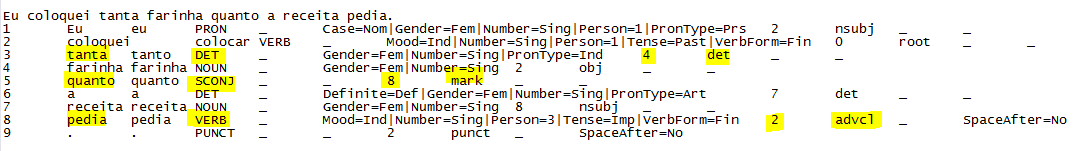
\includegraphics[width=\textwidth,height=\textheight,keepaspectratio]{imagesDrive/image20.png}
	    \caption{Eu coloquei \emph{tanta farinha quanto} a receita pedia}
	    \label{fig:comparative1}
	    \end{figure}{}
	
	\begin{figure}
	    \centering
	    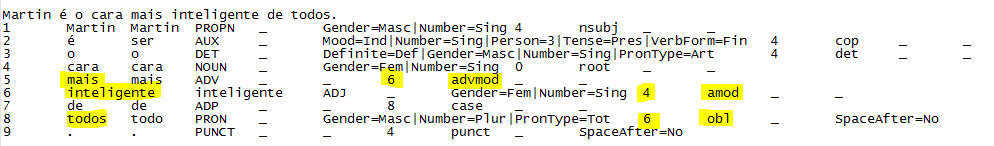
\includegraphics[width=\textwidth,height=\textheight,keepaspectratio]{imagesDrive/image27.png}
	    \caption{Martin é o cara \emph{mais inteligente de todos}}
	    \label{fig:comparative2}
	\end{figure}{}
	
	\subsection{Frases do Bosque-UD}

\section{Elementos discursivos}


	\subsection{É que}


	A construção \say{é que} pode aparecer de duas maneiras no corpus: marcada ou não como MWE. Como MWE, \say{é que} é uma ocorrência típica do discurso oral, sem ligação clara com a estrutura da oração. Por outro lado, \say{é} e \say{que} são independentes entre si quando introduzem uma oração subordinada substantiva predicativa ou subjetiva. (ver Xx)

Quando \say{é que} tem esse efeito discursivo, anota-se da seguinte maneira: \newline

		É: tem upos \emph{AUX} e deprel \emph{discourse}, e aponta para a head da oração; 

		Que: tem upos \emph{SCONJ} e deprel \emph{fixed}, e aponta para \say{é}. 

		\fullref{dep:equeMWE1}

		\fullref{fig:equeMWE2}

		\fullref{fig:equeMWE3}

OBS.: Consideramos \say{Não é que} como MWE.  

\say{\emph{Não é que} o sábio das matrizes encontrou, no PSD, entusiastas seguidores?} 


\begin{figure*}[htbp]
			\centering
			\vspace{.8cm}
			\begin{dependency}
				\begin{deptext}
					ADV \& ADV \& AUX \& SCONJ \& VERB \& DET \& NOUN \& SCONJ \& VERB \& DET \& NOUN \\
					Só \& depois \& é \& que \& levanto \& a \& cabeça \& para \& fazer \& um \& lançamento \\
					só \& depois \& ser \& que \& levantar \& o \& cabeça \& para \& fazer \& um \& lançamento \\
					\& \& \& \& MWE=é\_que \& \\
					\& \& \& \& MWEPOS=INTJ \& \\
				\end{deptext}
				\depedge{2}{1}{advmod}
				\depedge{5}{2}{advmod}
				\deproot{5}{3}{discourse}
				\depedge{3}{4}{fixed}
				\deproot{5}{root}
				\depedge{7}{6}{det}
				\depedge{5}{7}{obj}
				\depedge{9}{8}{mark}
				\depedge{5}{9}{advcl}
				\depedge{11}{10}{det}
				\depedge{9}{11}{obj}
				
			\end{dependency}
			\caption{Só depois \emph{é que} levanto a cabeça para fazer um lançamento}
			\label{dep:equeMWE1}
		\end{figure*}

		\begin{figure}
    	\centering
    	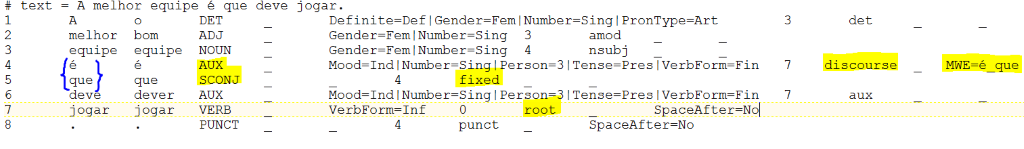
\includegraphics[width=\textwidth,height=\textheight,keepaspectratio]{imagesDrive/image16.png}
    	\caption{A melhor equipe \emph{é que} deve jogar}
    	\label{fig:equeMWE2}
    	\end{figure}{}

	\begin{figure}
    	\centering
    	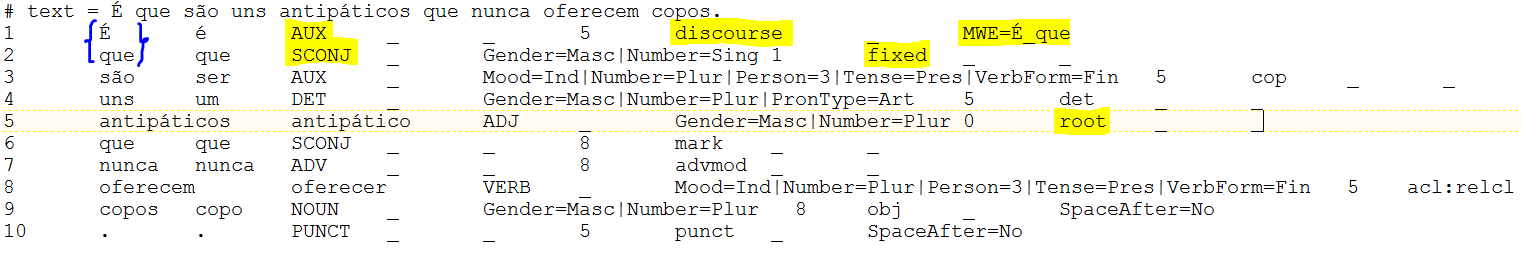
\includegraphics[width=\textwidth,height=\textheight,keepaspectratio]{imagesDrive/image71.PNG}
    	\caption{\emph{É que} são uns antipáticos que nunca oferecem copos}
    	\label{fig:equeMWE3}
    	\end{figure}{}

\chapter*{Apêndice}

	\hyperlink{toc}{Ir para tabela de conteúdos\\}

	Todas as listas são retiradas do corpus Bosque-UD em sua versão 2.5.
	
	\begin{table}[]
		\centering
		\begin{tabular}{|c|c|}
			\hline
			\textbf{Verbo de ligação} & \textbf{Frequência} \\\hline
			estar & 33\\\hline
			ser & 105\\\hline
		\end{tabular}
		\caption{Lista das 2 palavras que ocorrem 138 vezes como verbo de ligação (\emph{AUX/cop}) no Bosque-UD}
		\label{tab:verbosdeligacao}
	\end{table}

	\begin{table}[]
		\centering
		\begin{tabular}{|c|c|}
			\hline
			\textbf{Voz passiva} & \textbf{Frequência} \\\hline
			ficar & 1\\\hline
			ser & 1114\\\hline
		\end{tabular}
		\caption{Lista das 2 palavras que ocorrem 1115 vezes como voz passiva (\emph{AUX/aux:pass}) no Bosque-UD}
		\label{tab:vozpassiva}
	\end{table}

	\begin{table}[]
		\centering
		\begin{tabular}{|c|c|}
			\hline
			\textbf{Voz passiva} & \textbf{Frequência} \\\hline
			ficar & 1\\\hline
			ser & 1114\\\hline
		\end{tabular}
		\caption{Lista das 2 palavras que ocorrem 1115 vezes como locução verbal de tempo composto (\emph{AUX/aux}) no Bosque-UD}
		\label{tab:loctempocomposto}
	\end{table}

	\begin{table}[]
		\parbox{.45\linewidth}{
			\centering
			\begin{tabular}{|c|c|}
				\hline
				\textbf{MWE auxiliar} & \textbf{Frequência} \\\hline
				acabar de & 11\\\hline
				acabar por & 30\\\hline
				andar a & 3\\\hline
				chegar a & 22\\\hline
				começar a & 58\\\hline
				começar por & 6\\\hline
				continuar a & 57\\\hline
				continuar por & 1\\\hline
				deixar de & 30\\\hline
				dever a & 1\\\hline
				estar a & 124\\\hline
				estar para & 1\\\hline
				estar por & 1\\\hline
				ficar a & 4\\\hline
				ficar de & 1\\\hline
				haver a & 1\\\hline
				haver de & 2\\\hline
				haver que & 1\\\hline
				ir a & 3\\\hline
				ir de & 1\\\hline
				parar de & 3\\\hline
				passar a & 43\\\hline
				poder a & 3\\\hline
				ser de & 3\\\hline
				tender a & 1\\\hline
				ter a & 9\\\hline
				ter de & 62\\\hline
				ter que & 3\\\hline
				tornar a & 1\\\hline
				vir a & 42\\\hline
				voltar a & 42\\\hline
			\end{tabular}
		}
		\hfill
		\parbox{.45\linewidth}{
			\centering
			\begin{tabular}{|c|c|}
				\hline
				\textbf{MWE auxiliar} & \textbf{Frequência} \\\hline
				estar a & 124\\\hline
				ter de & 62\\\hline
				começar a & 58\\\hline
				continuar a & 57\\\hline
				passar a & 43\\\hline
				vir a & 42\\\hline
				voltar a & 42\\\hline
				acabar por & 30\\\hline
				deixar de & 30\\\hline
				chegar a & 22\\\hline
				acabar de & 11\\\hline
				ter a & 9\\\hline
				começar por & 6\\\hline
				ficar a & 4\\\hline
				andar a & 3\\\hline
				ir a & 3\\\hline
				parar de & 3\\\hline
				poder a & 3\\\hline
				ser de & 3\\\hline
				ter que & 3\\\hline
				haver de & 2\\\hline
				continuar por & 1\\\hline
				dever a & 1\\\hline
				estar para & 1\\\hline
				estar por & 1\\\hline
				ficar de & 1\\\hline
				haver a & 1\\\hline
				haver que & 1\\\hline
				ir de & 1\\\hline
				tender a & 1\\\hline
				tornar a & 1\\\hline
			\end{tabular}
		}
		\caption{Lista das 31 MWEs que ocorreriam 570 vezes como locuções auxiliares (\emph{AUX/aux + ADP/compound}) no Bosque-UD segundo nossa proposta de anotação}
		\label{tab:auxphrasalverb}
	\end{table}

	\begin{longtable}{ p{3cm} | p{1cm} | p{3cm} | p{1cm} }
		\hline
		\textbf{Primeiro verbo (ordem alfabética)} & \textbf{\#} & \textbf{Primeiro verbo (ordem de frequência)} & \textbf{\#} \\\hline
		abster & 2 & querer & 108\\\hline
		acabar & 3 & conseguir & 83\\\hline
		aceder & 1 & tentar & 64\\\hline
		aceitar & 6 & fazer & 45\\\hline
		achar & 5 & pretender & 39\\\hline
		aconselhar & 5 & permitir & 37\\\hline
		acreditar & 2 & decidir & 33\\\hline
		acusar & 30 & acusar & 30\\\hline
		admitir & 12 & deixar & 27\\\hline
		afirmar & 13 & procurar & 21\\\hline
		aguentar & 1 & levar & 20\\\hline
		ajudar & 9 & ver & 19\\\hline
		alegar & 3 & dar & 18\\\hline
		ambicionar & 1 & gostar & 17\\\hline
		ameaçar & 14 & obrigar & 17\\\hline
		andar & 2 & ser & 17\\\hline
		anunciar & 2 & saber & 16\\\hline
		aperceber & 1 & ameaçar & 14\\\hline
		apetecer & 1 & precisar & 14\\\hline
		aplicar & 1 & preferir & 14\\\hline
		apostar & 1 & resolver & 14\\\hline
		aprender & 5 & afirmar & 13\\\hline
		apresentar & 2 & admitir & 12\\\hline
		apressar & 1 & considerar & 12\\\hline
		aprestar & 1 & encontrar & 12\\\hline
		aproveitar & 1 & ter & 12\\\hline
		arriscar & 2 & dizer & 11\\\hline
		atender & 1 & destinar & 10\\\hline
		atrever & 1 & limitar & 10\\\hline
		autorizar & 3 & ajudar & 9\\\hline
		avisar & 1 & ficar & 9\\\hline
		bastar & 3 & preparar & 9\\\hline
		caber & 1 & esperar & 8\\\hline
		cansar & 1 & pensar & 8\\\hline
		cessar & 1 & comprometer & 7\\\hline
		chamar & 4 & consistir & 7\\\hline
		citar & 1 & continuar & 7\\\hline
		começar & 1 & convidar & 7\\\hline
		comprometer & 7 & recusar & 7\\\hline
		concordar & 3 & aceitar & 6\\\hline
		condenar & 1 & convencer & 6\\\hline
		conduzir & 1 & estar & 6\\\hline
		confidenciar & 1 & manter & 6\\\hline
		confirmar & 1 & prometer & 6\\\hline
		conseguir & 83 & achar & 5\\\hline
		considerar & 12 & aconselhar & 5\\\hline
		consistir & 7 & aprender & 5\\\hline
		consultar & 1 & forçar & 5\\\hline
		contar & 1 & mandar & 5\\\hline
		continuar & 7 & parecer & 5\\\hline
		contribuir & 3 & passar & 5\\\hline
		convencer & 6 & propor & 5\\\hline
		convencionar & 1 & tender & 5\\\hline
		convidar & 7 & visar & 5\\\hline
		credenciar & 1 & chamar & 4\\\hline
		criticar & 1 & desejar & 4\\\hline
		culpar & 1 & encarregar & 4\\\hline
		dar & 18 & evitar & 4\\\hline
		decidir & 33 & impedir & 4\\\hline
		declarar & 3 & interessar & 4\\\hline
		declinar & 1 & proibir & 4\\\hline
		dedicar & 2 & reconhecer & 4\\\hline
		deixar & 27 & sentir & 4\\\hline
		depender & 1 & tencionar & 4\\\hline
		desafiar & 2 & tratar & 4\\\hline
		desejar & 4 & acabar & 3\\\hline
		desistir & 1 & alegar & 3\\\hline
		destinar & 10 & autorizar & 3\\\hline
		dever & 3 & bastar & 3\\\hline
		dispor & 3 & concordar & 3\\\hline
		dizer & 11 & contribuir & 3\\\hline
		duvidar & 1 & declarar & 3\\\hline
		empenhar & 2 & dever & 3\\\hline
		encarregar & 4 & dispor & 3\\\hline
		encontrar & 12 & insistir & 3\\\hline
		ensinar & 1 & ir & 3\\\hline
		equivaler & 1 & optar & 3\\\hline
		escolher & 1 & ousar & 3\\\hline
		escusar & 2 & pôr & 3\\\hline
		esperar & 8 & vir & 3\\\hline
		estar & 6 & abster & 2\\\hline
		estimar & 1 & acreditar & 2\\\hline
		estimular & 1 & andar & 2\\\hline
		estudar & 1 & anunciar & 2\\\hline
		evitar & 4 & apresentar & 2\\\hline
		exigir & 1 & arriscar & 2\\\hline
		exortar & 1 & dedicar & 2\\\hline
		experimentar & 1 & desafiar & 2\\\hline
		falar & 2 & empenhar & 2\\\hline
		fartar & 1 & escusar & 2\\\hline
		fazer & 45 & falar & 2\\\hline
		ficar & 9 & garantir & 2\\\hline
		fingir & 1 & haver & 2\\\hline
		foi & 1 & imaginar & 2\\\hline
		forçar & 5 & impor & 2\\\hline
		garantir & 2 & importar & 2\\\hline
		gostar & 17 & incentivar & 2\\\hline
		habituar & 1 & mostrar & 2\\\hline
		haver & 2 & necessitar & 2\\\hline
		imaginar & 2 & negar & 2\\\hline
		impedir & 4 & ouvir & 2\\\hline
		impor & 2 & parar & 2\\\hline
		importar & 2 & queixar & 2\\\hline
		incentivar & 2 & receber & 2\\\hline
		incluir & 1 & referir & 2\\\hline
		indagar & 1 & resistir & 2\\\hline
		influenciar & 1 & sentar & 2\\\hline
		informar & 1 & tornar & 2\\\hline
		insinuar & 1 & aceder & 1\\\hline
		insistir & 3 & aguentar & 1\\\hline
		instar & 1 & ambicionar & 1\\\hline
		interessar & 4 & aperceber & 1\\\hline
		ir & 3 & apetecer & 1\\\hline
		lembrar & 1 & aplicar & 1\\\hline
		levar & 20 & apostar & 1\\\hline
		limitar & 10 & apressar & 1\\\hline
		mandar & 5 & aprestar & 1\\\hline
		manter & 6 & aproveitar & 1\\\hline
		merecer & 1 & atender & 1\\\hline
		mostrar & 2 & atrever & 1\\\hline
		necessitar & 2 & avisar & 1\\\hline
		negar & 2 & caber & 1\\\hline
		obrigar & 17 & cansar & 1\\\hline
		optar & 3 & cessar & 1\\\hline
		orgulhar & 1 & citar & 1\\\hline
		ousar & 3 & começar & 1\\\hline
		ouvir & 2 & condenar & 1\\\hline
		parar & 2 & conduzir & 1\\\hline
		parecer & 5 & confidenciar & 1\\\hline
		passado & 1 & confirmar & 1\\\hline
		passar & 5 & consultar & 1\\\hline
		pedir & 1 & contar & 1\\\hline
		pensar & 8 & convencionar & 1\\\hline
		perder & 1 & credenciar & 1\\\hline
		permanecer & 1 & criticar & 1\\\hline
		permitir & 37 & culpar & 1\\\hline
		persuadir & 1 & declinar & 1\\\hline
		planear & 1 & depender & 1\\\hline
		poder & 1 & desistir & 1\\\hline
		precisar & 14 & duvidar & 1\\\hline
		preferir & 14 & ensinar & 1\\\hline
		preparar & 9 & equivaler & 1\\\hline
		pretender & 39 & escolher & 1\\\hline
		prevenir & 1 & estimar & 1\\\hline
		prever & 1 & estimular & 1\\\hline
		procurar & 21 & estudar & 1\\\hline
		proibir & 4 & exigir & 1\\\hline
		projectar & 1 & exortar & 1\\\hline
		prometer & 6 & experimentar & 1\\\hline
		propiciar & 1 & fartar & 1\\\hline
		propor & 5 & fingir & 1\\\hline
		provocar & 1 & foi & 1\\\hline
		pôr & 3 & habituar & 1\\\hline
		queixar & 2 & incluir & 1\\\hline
		querer & 108 & indagar & 1\\\hline
		receber & 2 & influenciar & 1\\\hline
		reclamar & 1 & informar & 1\\\hline
		recomeçar & 1 & insinuar & 1\\\hline
		recompensar & 1 & instar & 1\\\hline
		reconhecer & 4 & lembrar & 1\\\hline
		recordar & 1 & merecer & 1\\\hline
		recusar & 7 & orgulhar & 1\\\hline
		reduzir & 1 & passado & 1\\\hline
		referir & 2 & pedir & 1\\\hline
		resistir & 2 & perder & 1\\\hline
		resolver & 14 & permanecer & 1\\\hline
		respeitar & 1 & persuadir & 1\\\hline
		restar & 1 & planear & 1\\\hline
		retirar & 1 & poder & 1\\\hline
		saber & 16 & prevenir & 1\\\hline
		salientar & 1 & prever & 1\\\hline
		sentar & 2 & projectar & 1\\\hline
		sentir & 4 & propiciar & 1\\\hline
		ser & 17 & provocar & 1\\\hline
		soar & 1 & reclamar & 1\\\hline
		sonhar & 1 & recomeçar & 1\\\hline
		sublinhar & 1 & recompensar & 1\\\hline
		sujeitar & 1 & recordar & 1\\\hline
		suportar & 1 & reduzir & 1\\\hline
		surgir & 1 & respeitar & 1\\\hline
		suspeitar & 1 & restar & 1\\\hline
		tardar & 1 & retirar & 1\\\hline
		teimar & 1 & salientar & 1\\\hline
		temer & 1 & soar & 1\\\hline
		tencionar & 4 & sonhar & 1\\\hline
		tender & 5 & sublinhar & 1\\\hline
		tentar & 64 & sujeitar & 1\\\hline
		ter & 12 & suportar & 1\\\hline
		tornar & 2 & surgir & 1\\\hline
		tratar & 4 & suspeitar & 1\\\hline
		trazer & 1 & tardar & 1\\\hline
		ver & 19 & teimar & 1\\\hline
		vir & 3 & temer & 1\\\hline
		virar & 1 & trazer & 1\\\hline
		visar & 5 & virar & 1\\\hline
		voltar & 1 & voltar & 1\\\hline
		\caption{Lista dos 196 verbos plenos que ocorrem 1150 vezes como \emph{pais} de uma colocação verbal no Bosque-UD}
		\label{tab:naolocverbal}
	\end{longtable}

	
\chapter*{Abreviações}

\hyperlink{toc}{Ir para tabela de conteúdos\\}



\chapter*{Agradecimentos}

\hyperlink{toc}{Ir para tabela de conteúdos\\}



\printbibliography[heading=subbibliography,notkeyword=this]

\end{document}
